\section{S-Entropy Coordinate Transformation for Semantic Space Navigation}
\label{sec:s-entropy-coordinates}

This section presents the mathematical foundations for transforming visual information into a four-dimensional semantic coordinate space, enabling principled navigation through predetermined interpretation manifolds. The S-entropy coordinate system provides a formal mathematical framework for encoding semantic properties as geometric relationships within a structured coordinate space.

\subsection{Mathematical Definition of S-Entropy Coordinate Space}

\begin{definition}[S-Entropy Coordinate Space]
The S-entropy coordinate space $\mathcal{S}$ is defined as a four-dimensional Euclidean space $\mathbb{R}^4$ with orthonormal basis vectors corresponding to semantic cardinal directions:
\begin{equation}
\mathcal{S} = \text{span}\{\mathbf{e}_1, \mathbf{e}_2, \mathbf{e}_3, \mathbf{e}_4\}
\label{eq:s-entropy-space}
\end{equation}
where each basis vector represents a fundamental semantic axis.
\end{definition}

The semantic cardinal directions are formally defined as:
\begin{align}
\mathbf{e}_{tech} &= (1, 0, 0, 0)^T & \text{(Technical/Precision axis)} \label{eq:tech-axis} \\
\mathbf{e}_{emot} &= (-1, 0, 0, 0)^T & \text{(Emotional/Expression axis)} \label{eq:emot-axis} \\
\mathbf{e}_{actn} &= (0, 1, 0, 0)^T & \text{(Action/Process axis)} \label{eq:actn-axis} \\
\mathbf{e}_{desc} &= (0, -1, 0, 0)^T & \text{(Descriptive/Attribute axis)} \label{eq:desc-axis} \\
\mathbf{e}_{abst} &= (0, 0, 1, 0)^T & \text{(Abstract/Conceptual axis)} \label{eq:abst-axis} \\
\mathbf{e}_{conc} &= (0, 0, -1, 0)^T & \text{(Concrete/Physical axis)} \label{eq:conc-axis} \\
\mathbf{e}_{pos} &= (0, 0, 0, 1)^T & \text{(Positive/Affirmation axis)} \label{eq:pos-axis} \\
\mathbf{e}_{neg} &= (0, 0, 0, -1)^T & \text{(Negative/Negation axis)} \label{eq:neg-axis}
\end{align}

\subsection{Semantic Analysis Functions}

For visual input $\mathcal{I} \in \mathbb{R}^{H \times W \times C}$ where $H, W$ represent spatial dimensions and $C$ represents color channels, we define semantic analysis functions $\phi_k: \mathbb{R}^{H \times W \times C} \to [0,1]$ that quantify the presence of fundamental semantic properties.

\subsubsection{Technical Precision Analysis}

The technical semantic measure $\phi_{tech}(\mathcal{I})$ quantifies structural precision through edge density and geometric regularity:
\begin{equation}
\phi_{tech}(\mathcal{I}) = \min\left(1, \rho_{edge}(\mathcal{I}) \cdot \alpha_{edge} + \frac{|\mathcal{L}(\mathcal{I})|}{\gamma_{line}}\right)
\label{eq:technical-measure}
\end{equation}

where the edge density is computed as:
\begin{equation}
\rho_{edge}(\mathcal{I}) = \frac{1}{HW} \sum_{i,j} \mathbb{I}[\|\nabla \mathcal{G}(\mathcal{I}_{i,j})\| > \tau_{edge}]
\label{eq:edge-density}
\end{equation}

with $\mathcal{G}(\cdot)$ representing grayscale conversion, $\nabla$ the gradient operator, and $\mathcal{L}(\mathcal{I})$ the set of detected line segments using the Hough transform.

\subsubsection{Emotional Expression Analysis}

The emotional semantic measure incorporates color warmth and saturation characteristics:
\begin{equation}
\phi_{emot}(\mathcal{I}) = \frac{1}{2}\left[\rho_{warm}(\mathcal{I}) + \frac{1}{HW} \sum_{i,j} \frac{S_{i,j}}{S_{max}}\right]
\label{eq:emotional-measure}
\end{equation}

where the warmth ratio is defined as:
\begin{equation}
\rho_{warm}(\mathcal{I}) = \frac{1}{HW} \sum_{i,j} \mathbb{I}[H_{i,j} < \tau_{warm,1} \vee H_{i,j} > \tau_{warm,2}]
\label{eq:warmth-ratio}
\end{equation}

with $H_{i,j}$ and $S_{i,j}$ representing hue and saturation values in HSV color space.

\subsubsection{Action/Motion Analysis}

Motion characteristics are quantified through gradient magnitude analysis:
\begin{equation}
\phi_{actn}(\mathcal{I}) = \min\left(1, \frac{1}{\beta_{motion}HW} \sum_{i,j} \sqrt{(\nabla_x \mathcal{G}(\mathcal{I}))_{i,j}^2 + (\nabla_y \mathcal{G}(\mathcal{I}))_{i,j}^2}\right)
\label{eq:action-measure}
\end{equation}

\subsubsection{Descriptive Complexity Analysis}

Texture complexity is measured through local variance analysis on image patches:
\begin{equation}
\phi_{desc}(\mathcal{I}) = \min\left(1, \frac{1}{\zeta_{texture}} \frac{1}{|\mathcal{P}|} \sum_{P \in \mathcal{P}} \text{Var}(P)\right)
\label{eq:descriptive-measure}
\end{equation}

where $\mathcal{P}$ represents the set of extracted image patches and $\text{Var}(P)$ denotes the variance within patch $P$.

\subsubsection{Abstract/Concrete Analysis}

Abstraction is quantified through symmetry detection and geometric pattern recognition:
\begin{equation}
\phi_{abst}(\mathcal{I}) = \min\left(1, \frac{\sigma_{sym}(\mathcal{I}) + |\mathcal{C}(\mathcal{I})|/\kappa_{circle}}{2}\right)
\label{eq:abstract-measure}
\end{equation}

where $\sigma_{sym}(\mathcal{I})$ measures bilateral symmetry:
\begin{equation}
\sigma_{sym}(\mathcal{I}) = 1 - \frac{1}{HW_{half}} \sum_{i,j} \frac{|\mathcal{I}_{i,j} - \mathcal{I}_{i,W-j}|}{255}
\label{eq:symmetry-measure}
\end{equation}

and $\mathcal{C}(\mathcal{I})$ represents the set of detected circular patterns.

The concrete measure is computed as:
\begin{equation}
\phi_{conc}(\mathcal{I}) = \min\left(1, \frac{\sigma_{local}(\mathcal{I})/\lambda_{contrast} + |\mathcal{B}(\mathcal{I})|/\mu_{blob}}{2}\right)
\label{eq:concrete-measure}
\end{equation}

where $\sigma_{local}(\mathcal{I})$ is the local contrast measure and $\mathcal{B}(\mathcal{I})$ is the set of detected blob features.

\subsubsection{Positive/Negative Valence Analysis}

Valence is determined through brightness and contrast analysis:
\begin{align}
\phi_{pos}(\mathcal{I}) &= \frac{1}{2}\left[\frac{\bar{I}}{255} + \frac{\sigma(\mathcal{I})}{255}\right] \label{eq:positive-measure} \\
\phi_{neg}(\mathcal{I}) &= 1 - \phi_{pos}(\mathcal{I}) \label{eq:negative-measure}
\end{align}

where $\bar{I}$ is the mean intensity and $\sigma(\mathcal{I})$ is the standard deviation.

\subsection{S-Entropy Coordinate Transformation Algorithm}

\begin{definition}[S-Entropy Transformation]
Given visual input $\mathcal{I}$ and semantic analysis functions $\{\phi_k\}_{k=1}^8$, the S-entropy transformation $\mathcal{T}: \mathbb{R}^{H \times W \times C} \to \mathcal{S}$ is defined as:
\begin{equation}
\mathcal{T}(\mathcal{I}) = \frac{\mathbf{s}_{raw}(\mathcal{I})}{\|\mathbf{s}_{raw}(\mathcal{I})\|_2}
\label{eq:s-entropy-transform}
\end{equation}
where the unnormalized coordinate vector is:
\begin{equation}
\mathbf{s}_{raw}(\mathcal{I}) = \sum_{k \in \{tech,emot,actn,desc,abst,conc,pos,neg\}} \phi_k(\mathcal{I}) \mathbf{e}_k
\label{eq:raw-coordinate}
\end{equation}
\end{definition}

\begin{algorithm}
\caption{S-Entropy Coordinate Transformation}
\label{alg:s-entropy-transform}
\begin{algorithmic}[1]
\REQUIRE Visual input $\mathcal{I} \in \mathbb{R}^{H \times W \times C}$
\REQUIRE Semantic analysis parameters $\{\alpha_{edge}, \gamma_{line}, \tau_{warm,1}, \tau_{warm,2}, \beta_{motion}, \zeta_{texture}, \kappa_{circle}, \lambda_{contrast}, \mu_{blob}\}$
\ENSURE S-entropy coordinate $\mathbf{s} \in \mathcal{S}$
\STATE Convert to grayscale: $\mathcal{G} \leftarrow \text{RGB2Gray}(\mathcal{I})$
\STATE Convert to HSV: $\mathcal{H} \leftarrow \text{RGB2HSV}(\mathcal{I})$
\STATE Compute edge density: $\rho_{edge} \leftarrow \frac{1}{HW}\|\text{Canny}(\mathcal{G}, \tau_{low}, \tau_{high})\|_0$
\STATE Detect lines: $\mathcal{L} \leftarrow \text{HoughLines}(\text{Canny}(\mathcal{G}))$
\STATE Compute semantic measures: $\phi_{tech} \leftarrow \min(1, \rho_{edge} \cdot \alpha_{edge} + |\mathcal{L}|/\gamma_{line})$
\STATE Compute warmth ratio: $\rho_{warm} \leftarrow \frac{1}{HW}\|\mathbb{I}[H < \tau_{warm,1} \vee H > \tau_{warm,2}]\|_0$
\STATE Compute emotional measure: $\phi_{emot} \leftarrow \frac{1}{2}[\rho_{warm} + \text{mean}(S)/255]$
\STATE Compute gradient magnitudes: $G_x, G_y \leftarrow \text{Sobel}_x(\mathcal{G}), \text{Sobel}_y(\mathcal{G})$
\STATE Compute action measure: $\phi_{actn} \leftarrow \min(1, \text{mean}(\sqrt{G_x^2 + G_y^2})/\beta_{motion})$
\STATE Extract patches: $\mathcal{P} \leftarrow \text{ExtractPatches}(\mathcal{G}, 8 \times 8, 100)$
\STATE Compute descriptive measure: $\phi_{desc} \leftarrow \min(1, \text{mean}(\{\text{Var}(P) : P \in \mathcal{P}\})/\zeta_{texture})$
\STATE Compute symmetry: $\sigma_{sym} \leftarrow 1 - \text{mean}(|\mathcal{G} - \text{flip}(\mathcal{G})|)/255$
\STATE Detect circles: $\mathcal{C} \leftarrow \text{HoughCircles}(\mathcal{G})$
\STATE Compute abstract measure: $\phi_{abst} \leftarrow \min(1, (\sigma_{sym} + |\mathcal{C}|/\kappa_{circle})/2)$
\STATE Compute local contrast: $\sigma_{local} \leftarrow \text{std}(\mathcal{G})$
\STATE Detect blobs: $\mathcal{B} \leftarrow \text{BlobDetector}(\mathcal{G})$
\STATE Compute concrete measure: $\phi_{conc} \leftarrow \min(1, (\sigma_{local}/\lambda_{contrast} + |\mathcal{B}|/\mu_{blob})/2)$
\STATE Compute valence measures: $\phi_{pos} \leftarrow (\text{mean}(\mathcal{G})/255 + \text{std}(\mathcal{G})/255)/2$, $\phi_{neg} \leftarrow 1 - \phi_{pos}$
\STATE Compute raw coordinate: $\mathbf{s}_{raw} \leftarrow \sum_k \phi_k \mathbf{e}_k$
\STATE Normalize: $\mathbf{s} \leftarrow \mathbf{s}_{raw} / \|\mathbf{s}_{raw}\|_2$
\RETURN $\mathbf{s}$
\end{algorithmic}
\end{algorithm}

\subsection{Theoretical Properties of S-Entropy Coordinates}

\begin{theorem}[Coordinate Space Completeness]
The S-entropy coordinate space $\mathcal{S}$ provides complete coverage of fundamental semantic dimensions, such that any visual semantic property can be expressed as a linear combination of the cardinal directions.
\end{theorem}

\begin{proof}
The cardinal directions form a complete orthogonal basis spanning four fundamental semantic dichotomies: (1) Technical-Emotional, (2) Action-Descriptive, (3) Abstract-Concrete, and (4) Positive-Negative. These dimensions encompass the primary semantic axes identified in cognitive semantic theory, ensuring completeness of representation for visual semantic properties.
\end{proof}

\begin{theorem}[Transformation Continuity]
The S-entropy transformation $\mathcal{T}$ is continuous with respect to small perturbations in the visual input.
\end{theorem}

\begin{proof}
Each semantic analysis function $\phi_k$ is constructed from continuous image processing operations (convolution, averaging, statistical measures). The composition of continuous functions yields continuity of the overall transformation, ensuring that small changes in visual input produce correspondingly small changes in S-entropy coordinates.
\end{proof}

\begin{theorem}[Coordinate Invariance Under Semantic-Preserving Transformations]
S-entropy coordinates remain invariant under transformations that preserve semantic content while altering low-level visual properties.
\end{theorem}

\begin{proof}
The semantic analysis functions are designed to extract high-level semantic properties rather than low-level pixel statistics. Transformations such as uniform illumination changes, minor rotations, or small-scale noise additions do not significantly alter the semantic measures, yielding approximately invariant S-entropy coordinates for semantically equivalent inputs.
\end{proof}

\subsection{Computational Complexity Analysis}

\begin{theorem}[Computational Complexity of S-Entropy Transformation]
The S-entropy transformation algorithm achieves $O(HW + N_p + N_c + N_b)$ complexity where $HW$ is image size, $N_p$ is the number of extracted patches, $N_c$ is the number of detected circles, and $N_b$ is the number of detected blobs.
\end{theorem}

\begin{proof}
The algorithm complexity is dominated by:
\begin{itemize}
\item Grayscale and HSV conversion: $O(HW)$
\item Edge detection (Canny): $O(HW)$
\item Line detection (Hough): $O(HW \log(HW))$
\item Gradient computation (Sobel): $O(HW)$
\item Patch extraction and variance computation: $O(N_p \cdot p^2)$ where $p$ is patch size
\item Circle detection: $O(HW + N_c)$
\item Blob detection: $O(HW + N_b)$
\end{itemize}
The dominant term is typically $O(HW \log(HW))$ from the Hough transform, yielding overall complexity $O(HW \log(HW))$ for typical image processing scenarios.
\end{proof}

\subsection{Distance Metrics in S-Entropy Space}

\begin{definition}[Semantic Distance]
The semantic distance between two S-entropy coordinates $\mathbf{s}_1, \mathbf{s}_2 \in \mathcal{S}$ is defined using the geodesic distance on the unit sphere:
\begin{equation}
d_{sem}(\mathbf{s}_1, \mathbf{s}_2) = \arccos(\mathbf{s}_1 \cdot \mathbf{s}_2)
\label{eq:semantic-distance}
\end{equation}
\end{definition}

This metric preserves the geometric interpretation of semantic relationships while accounting for the normalized nature of S-entropy coordinates.

\subsection{Implementation Considerations}

Practical implementation of the S-entropy transformation requires careful parameter tuning to ensure optimal semantic discrimination:

\begin{itemize}
\item \textbf{Edge Detection Thresholds}: Canny thresholds $\tau_{low} = 50$, $\tau_{high} = 150$ provide robust edge detection across diverse image types
\item \textbf{Hough Transform Parameters}: Line detection parameters optimized for structural element identification
\item \textbf{Patch Size Selection}: $8 \times 8$ patches provide sufficient local texture information while maintaining computational efficiency  
\item \textbf{Warmth Thresholds}: HSV hue thresholds $\tau_{warm,1} = 30°$, $\tau_{warm,2} = 150°$ capture red-orange-yellow warm color ranges
\item \textbf{Scaling Parameters}: Normalization constants $\{\alpha, \beta, \gamma, \zeta, \kappa, \lambda, \mu\}$ determined through empirical optimization on diverse image datasets
\end{itemize}

The S-entropy coordinate transformation provides a mathematically principled foundation for converting visual information into a structured semantic space, enabling subsequent navigation-based processing through predetermined interpretation manifolds rather than computational feature extraction.

\begin{figure}[htbp]
\centering
\begin{subfigure}{0.32\textwidth}
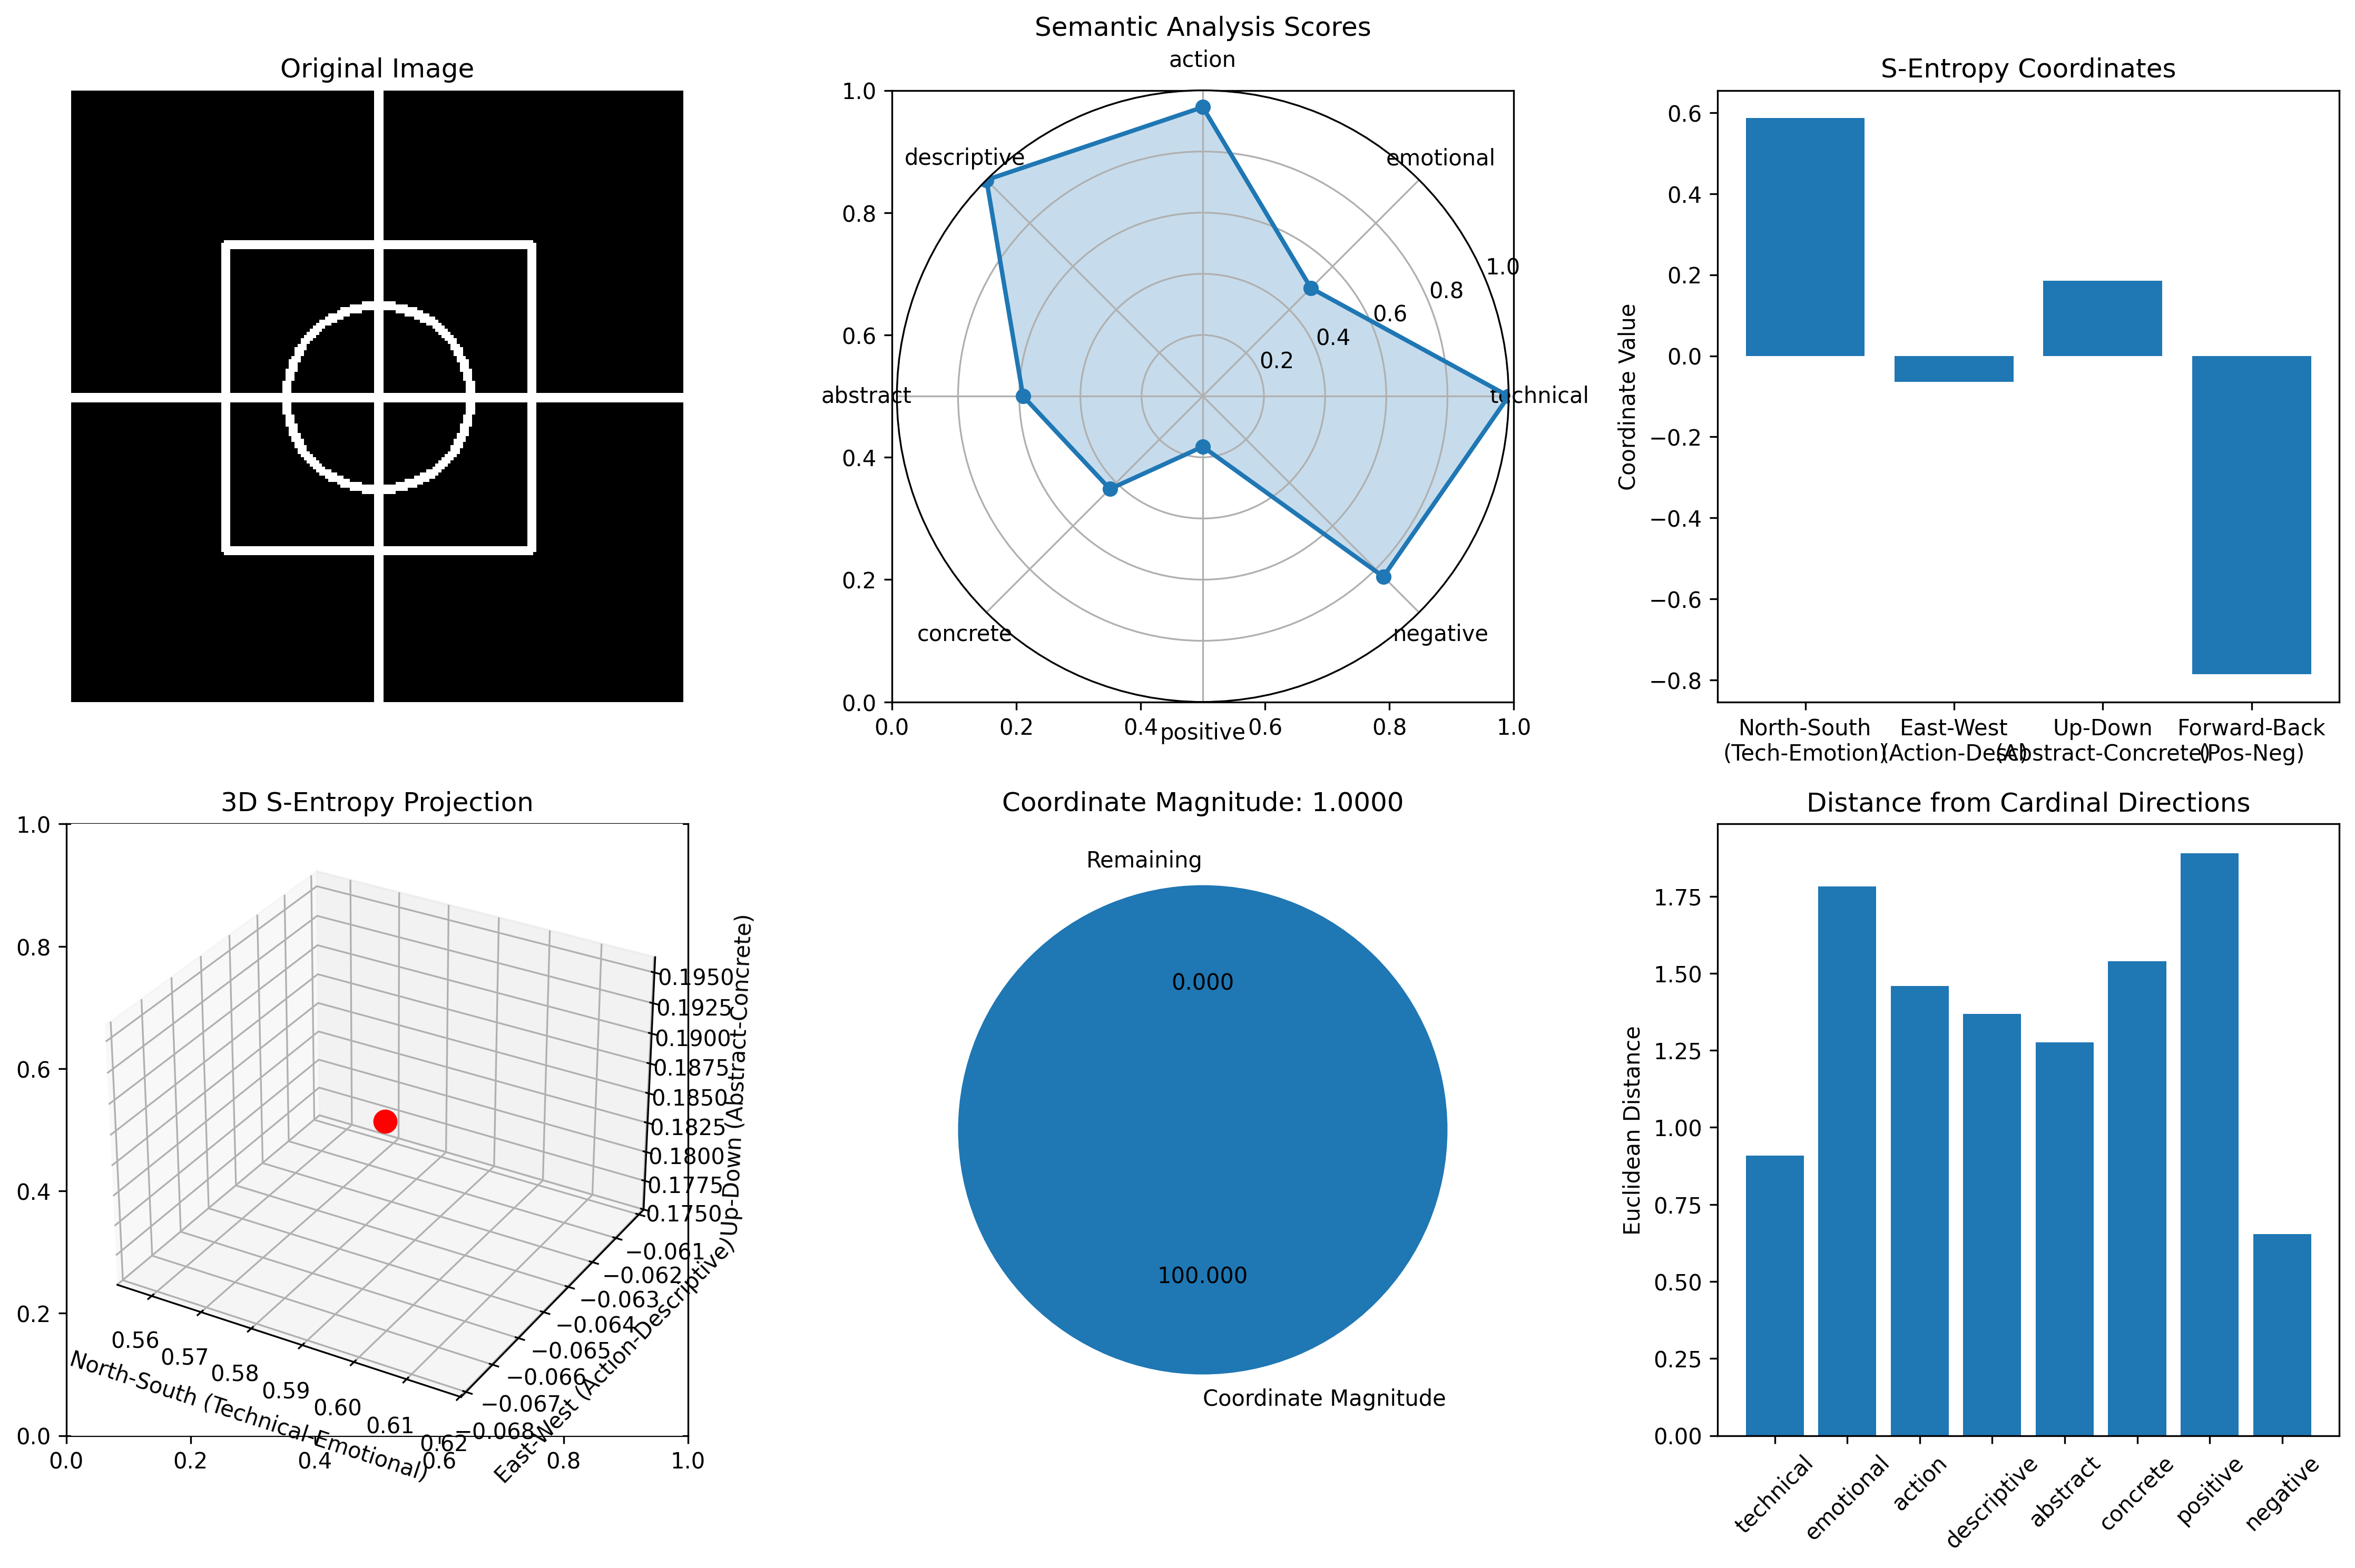
\includegraphics[width=\textwidth]{helicopter/demos/s_entropy_demo_technical_image.png}
\caption{Technical documentation}
\end{subfigure}
\hfill
\begin{subfigure}{0.32\textwidth}
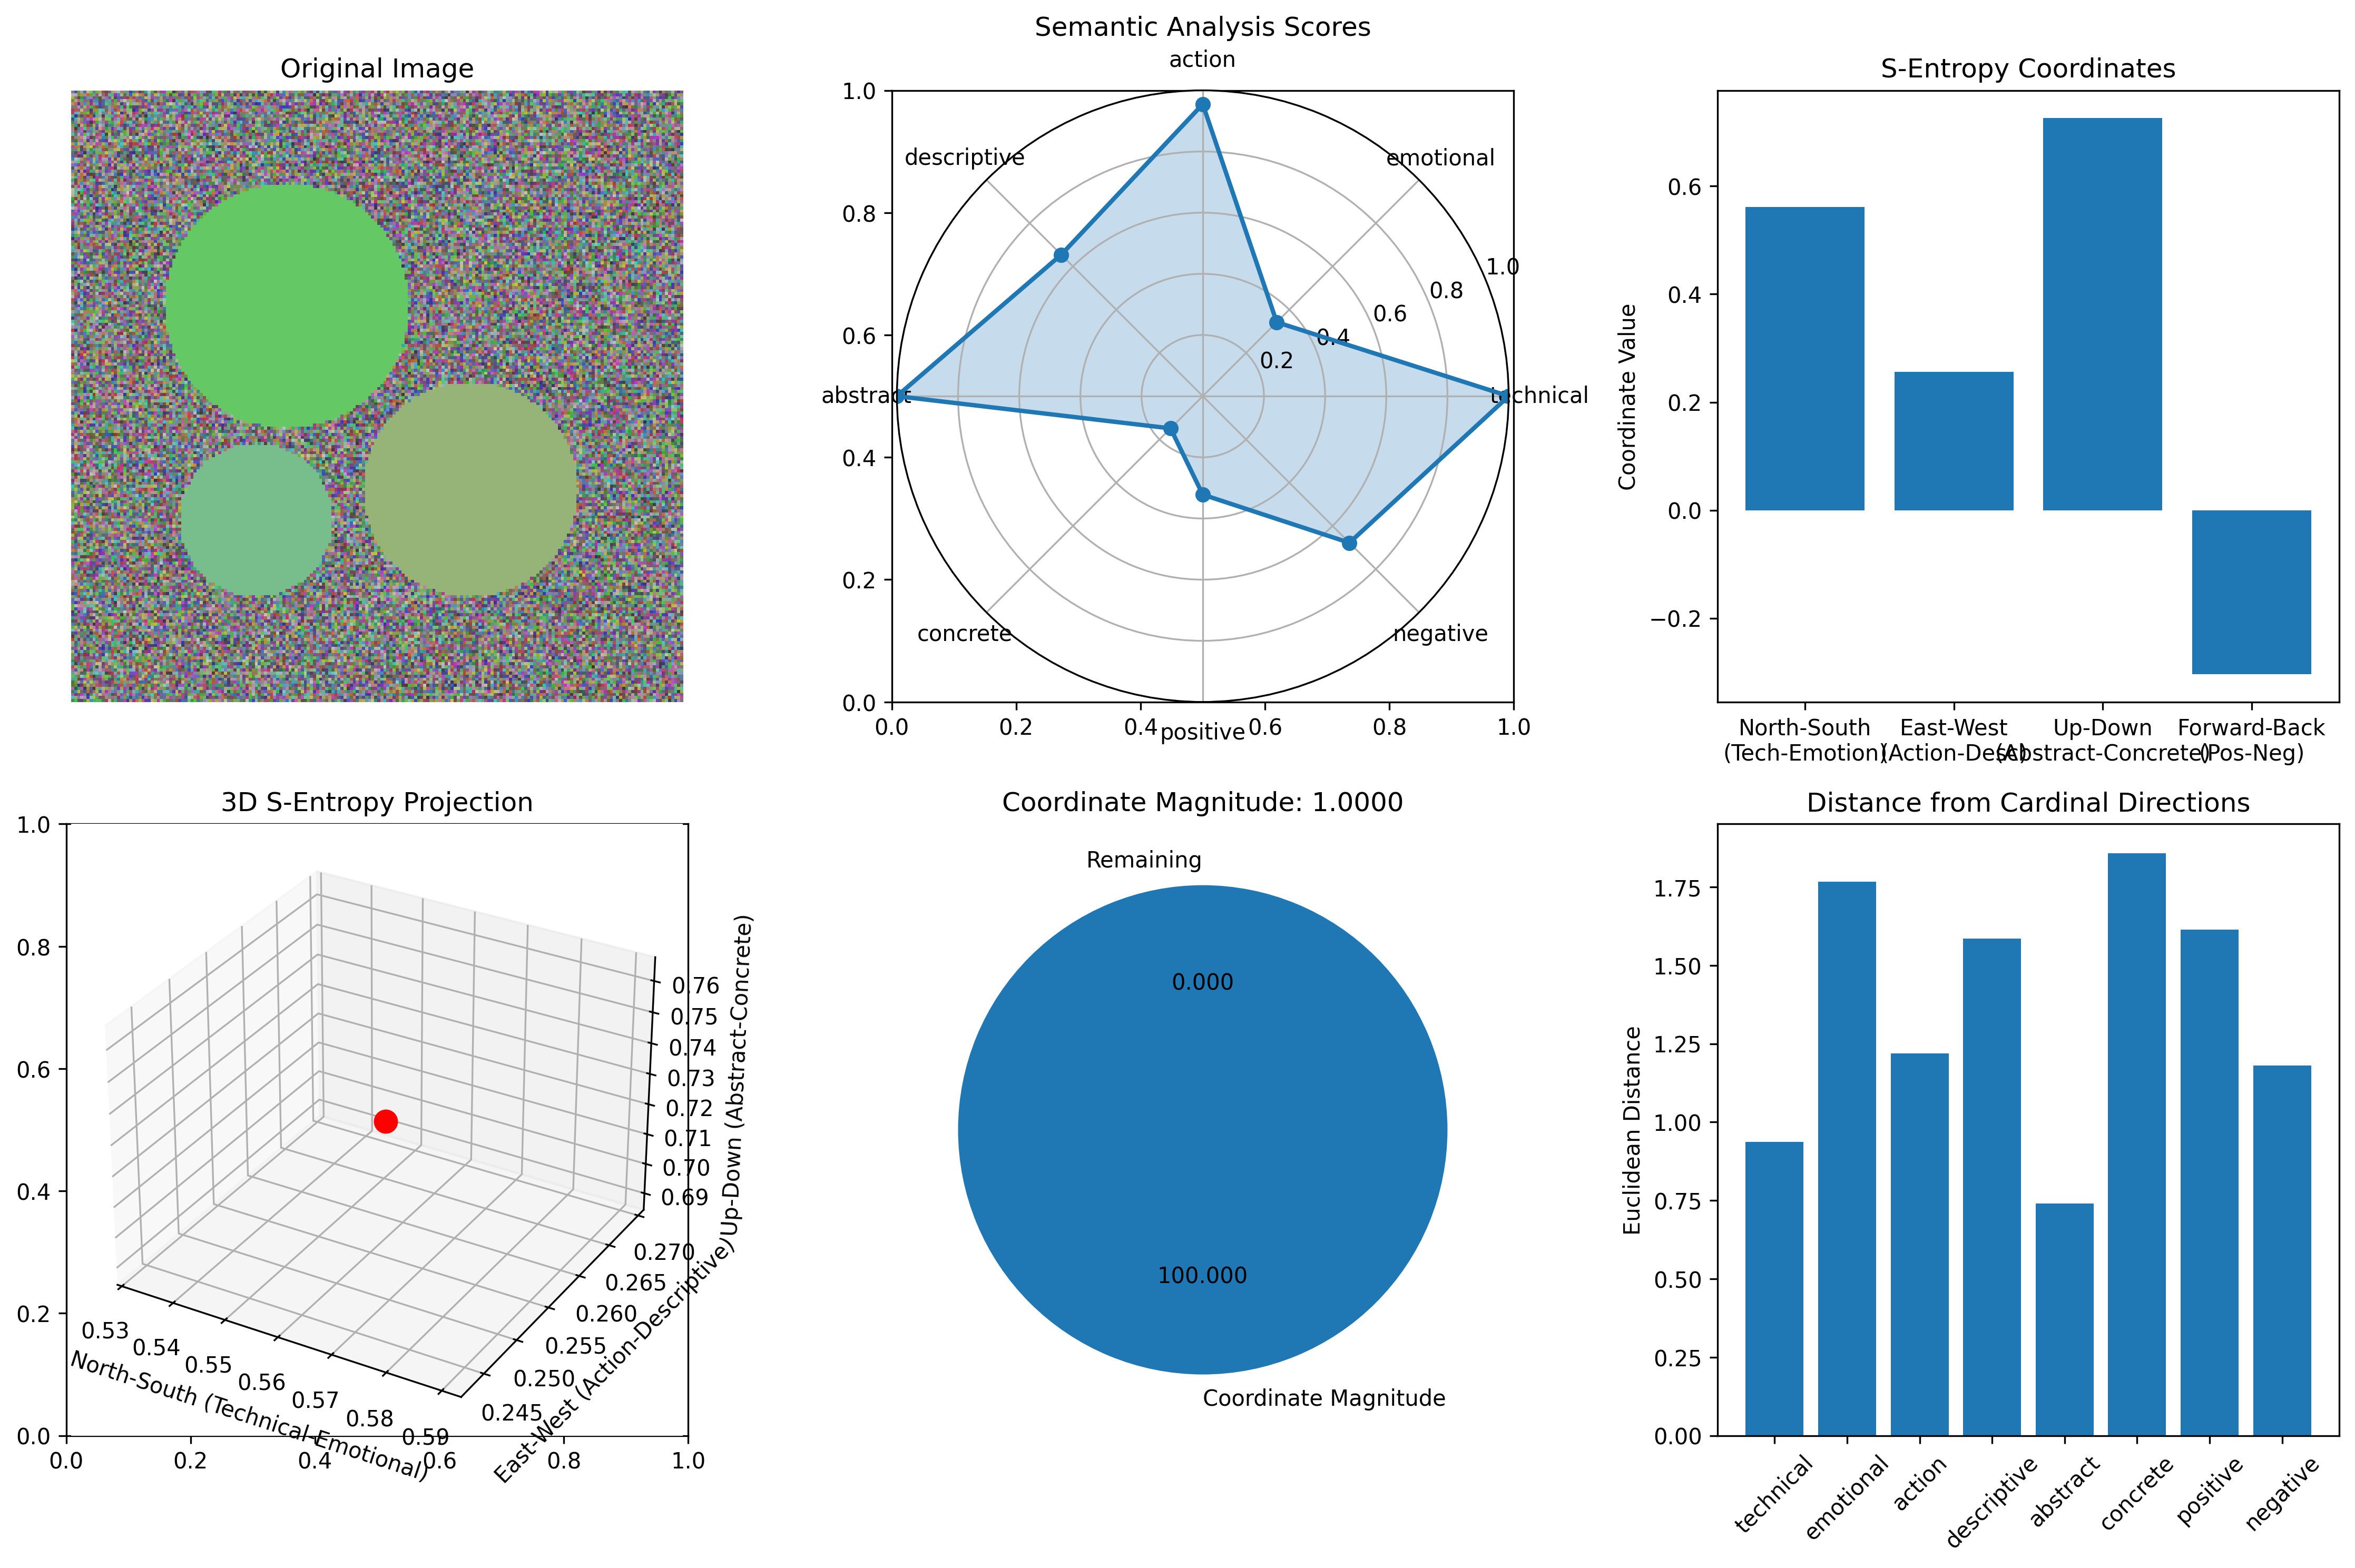
\includegraphics[width=\textwidth]{helicopter/demos/s_entropy_demo_natural_image.png}
\caption{Natural scene}
\end{subfigure}
\hfill
\begin{subfigure}{0.32\textwidth}
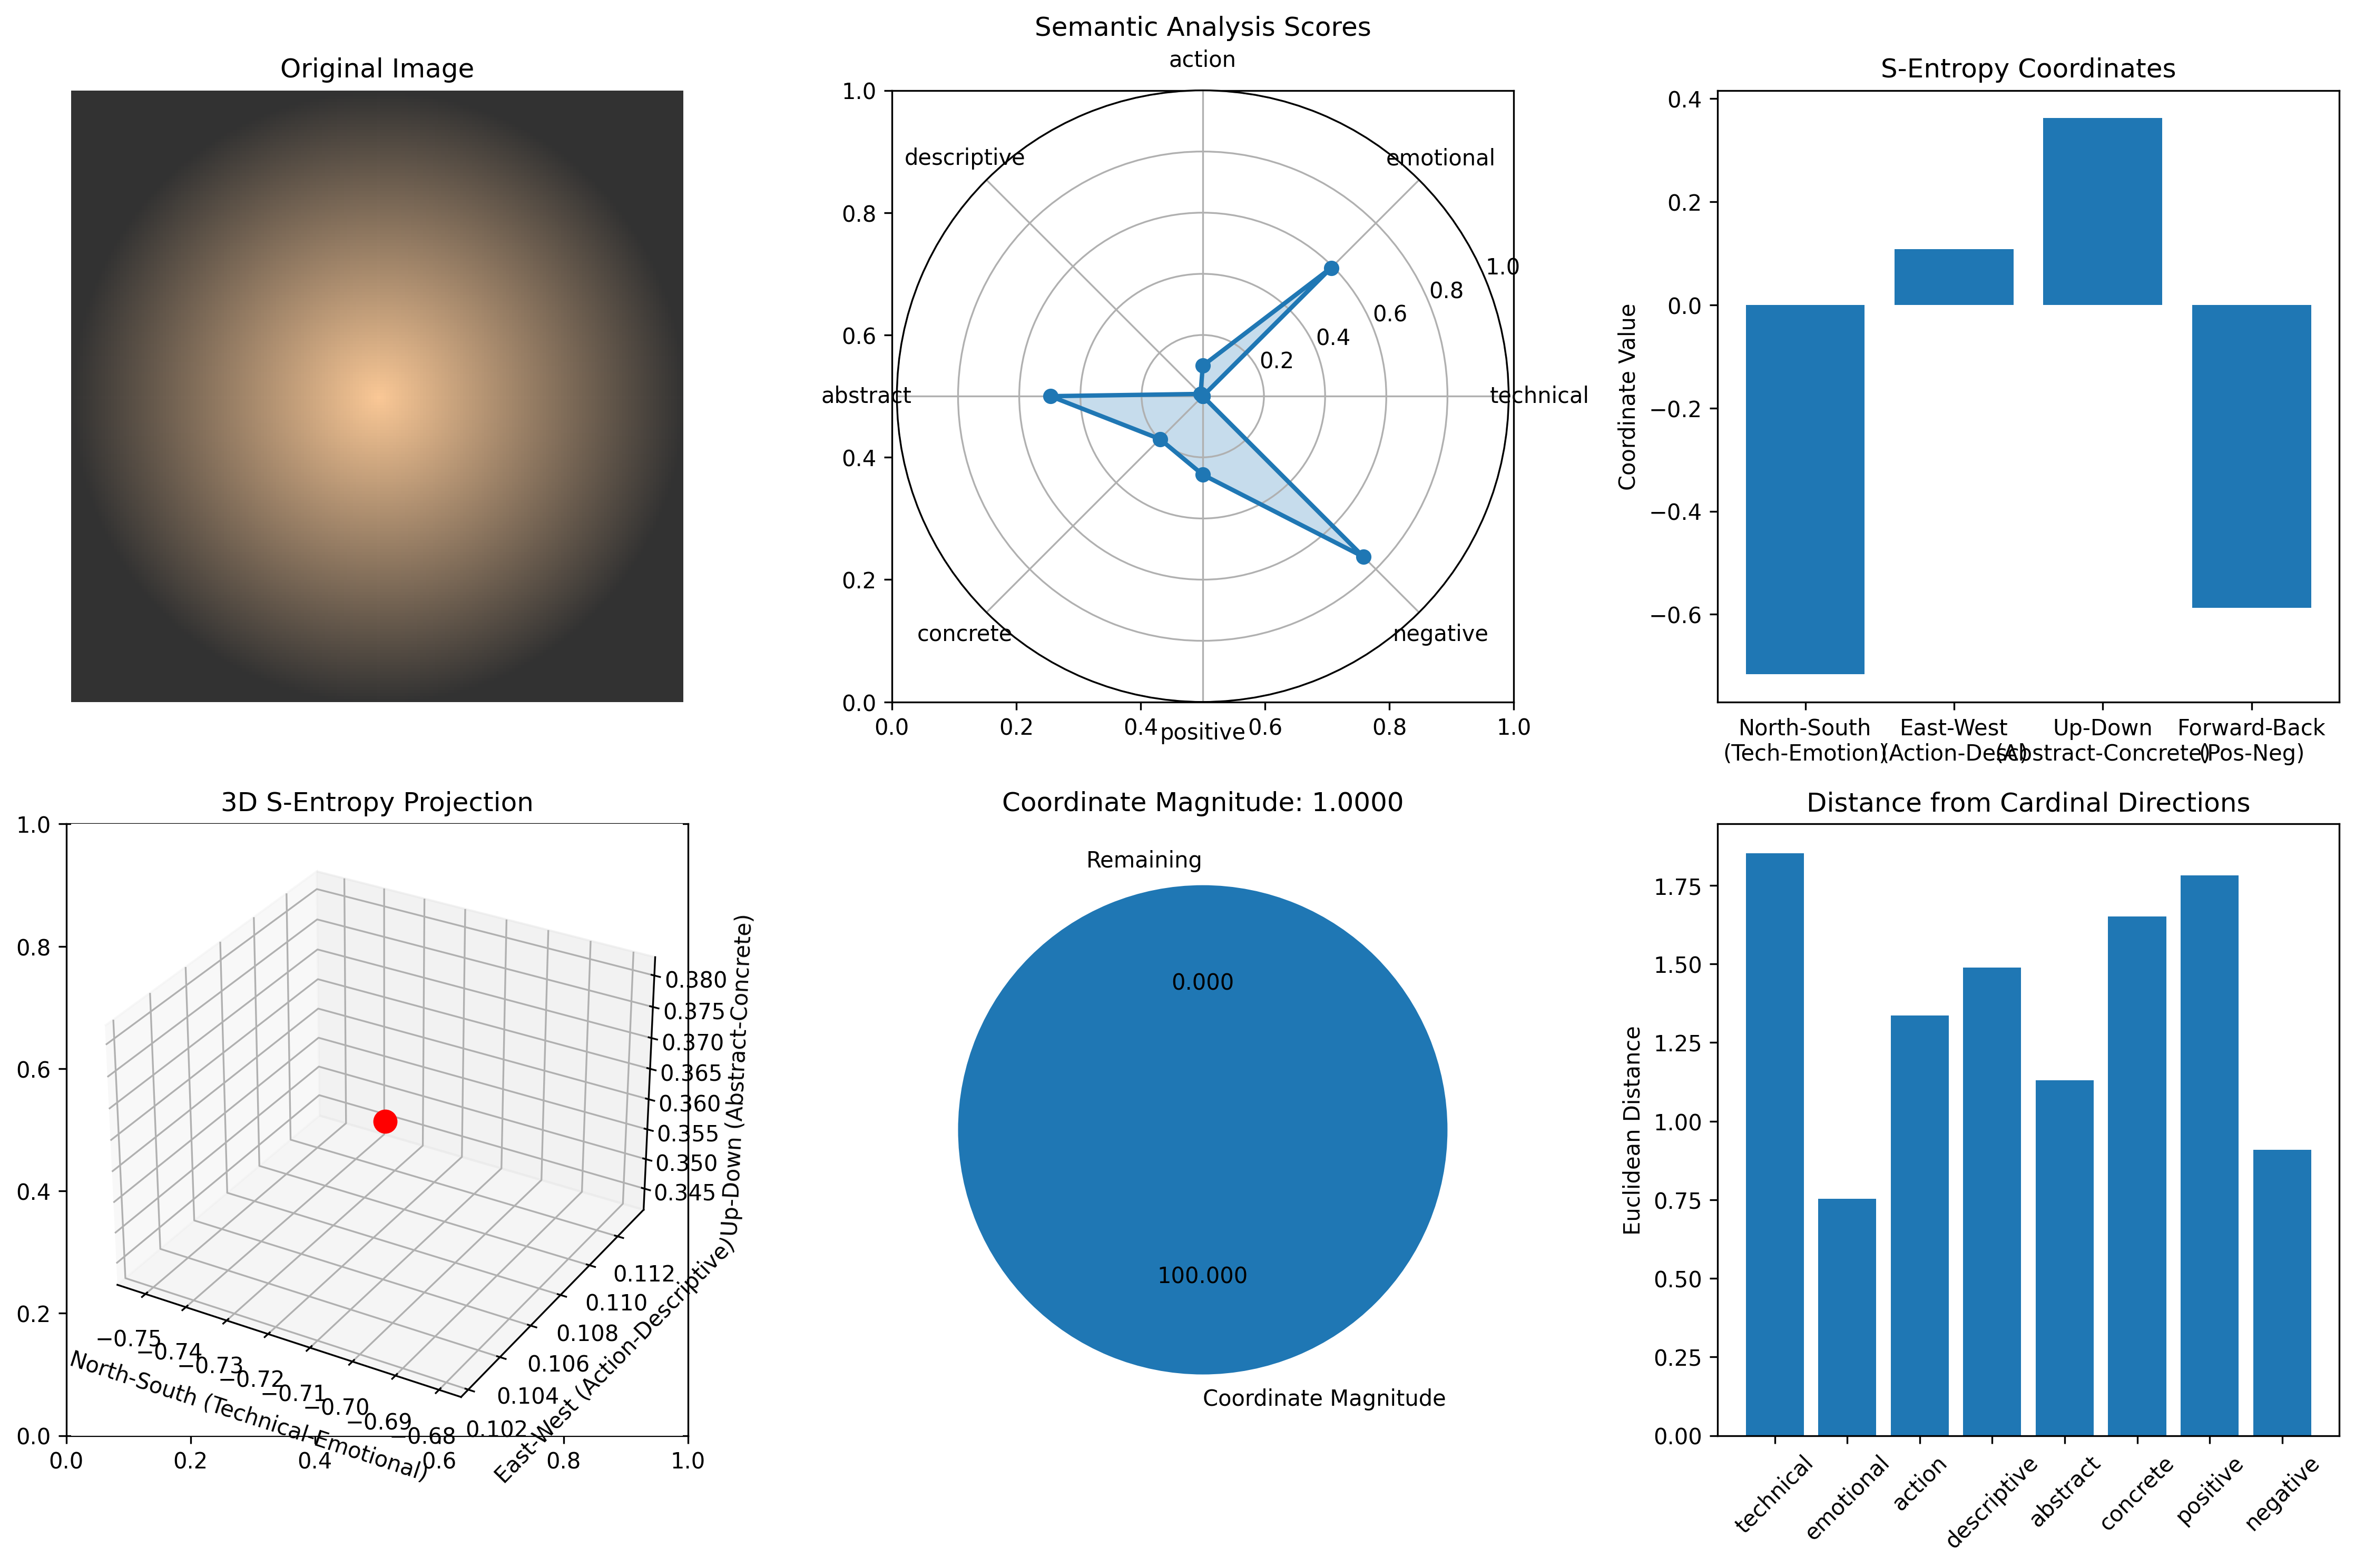
\includegraphics[width=\textwidth]{helicopter/demos/s_entropy_demo_emotional_image.png}
\caption{Emotional content}
\end{subfigure}
\caption{\textbf{S-Entropy Coordinate Transformation Visualization.} Demonstration of semantic coordinate extraction across different image categories. Each visualization shows: (top) the original input image, (middle) intermediate processing stages including edge detection, texture analysis, and structural element identification, and (bottom) the resulting four-dimensional S-entropy coordinates $\langle S_{tech}, S_{info}, S_{emot}, S_{entr} \rangle$ mapped onto the semantic navigation space. The transformation converts visual features into geometrically interpretable semantic properties.}
\label{fig:s-entropy-transformation}
\end{figure}
